\section{Results}
\label{sec:results}
\subsection{Discrimination of the five-fold probability ensembles}
All 15 principal seed-44 runs completed training and formal evaluation; the supplementary mean-pooling model contributed five further completed runs. Twenty evaluation receipts and their 60 registered report identities were verified. Each variant was evaluated by averaging its five fold probabilities for each of the same 175 holdout patients, including 56 positive outcomes, before computing any pCR metric. Macro equally averages the T0, T1, and T2 metrics.
\begin{table*}[t]
\centering
\small
\caption{Performance on the fixed internal holdout (175 patients, 56 pCR positive). For each patient and landmark, the five seed44 fold-model probabilities are averaged before computing any metric. Macro averages T0--T2 metrics. AP denotes average precision; F1 uses threshold 0.5. Entries are point estimates; paired differences, patient intervals, and multiplicity-adjusted significance are reported in Table~\ref{tab:bootstrap}.}
\label{tab:main}
\begin{tabular}{llrrr}
\toprule
Model & Landmark & AUROC & AP & F1 \\
\midrule
NoJEPA & T0 & 0.7275 & 0.5954 & 0.5354 \\
NoJEPA & T1 & 0.7281 & 0.5981 & 0.5426 \\
NoJEPA & T2 & 0.7281 & 0.5971 & 0.5469 \\
NoJEPA & Macro & 0.7279 & 0.5968 & 0.5416 \\
DirectReadout & T0 & 0.7372 & 0.6025 & 0.5669 \\
DirectReadout & T1 & 0.7416 & 0.6115 & 0.5692 \\
DirectReadout & T2 & 0.7410 & 0.6086 & 0.5672 \\
DirectReadout & Macro & 0.7399 & 0.6075 & 0.5678 \\
ForecastAttention & T0 & 0.7450 & 0.6256 & 0.5736 \\
ForecastAttention & T1 & 0.7521 & 0.6278 & 0.5442 \\
ForecastAttention & T2 & 0.7550 & 0.6315 & 0.5634 \\
ForecastAttention & Macro & 0.7507 & 0.6283 & 0.5604 \\
\bottomrule
\end{tabular}
\end{table*}


\fullmodel{} achieved AUROCs of 0.7450, 0.7521, and 0.7550 at T0, T1, and T2, with AP values of 0.6256, 0.6278, and 0.6315 (Fig.~\ref{fig:discrimination}). Its macro AUROC/AP/F1 was 0.7507/0.6283/0.5604, compared with 0.7279/0.5968/0.5416 for \nojepa{} and 0.7399/0.6075/0.5678 for \direct{}. Thus the full model had the highest AUROC and AP at every landmark among the principal variants, while \direct{} had higher macro F1. The full model's F1 was higher at T0 (0.5736 versus 0.5669), but lower at T1 (0.5442 versus 0.5692) and T2 (0.5634 versus 0.5672).

\begin{figure*}[t]
\centering
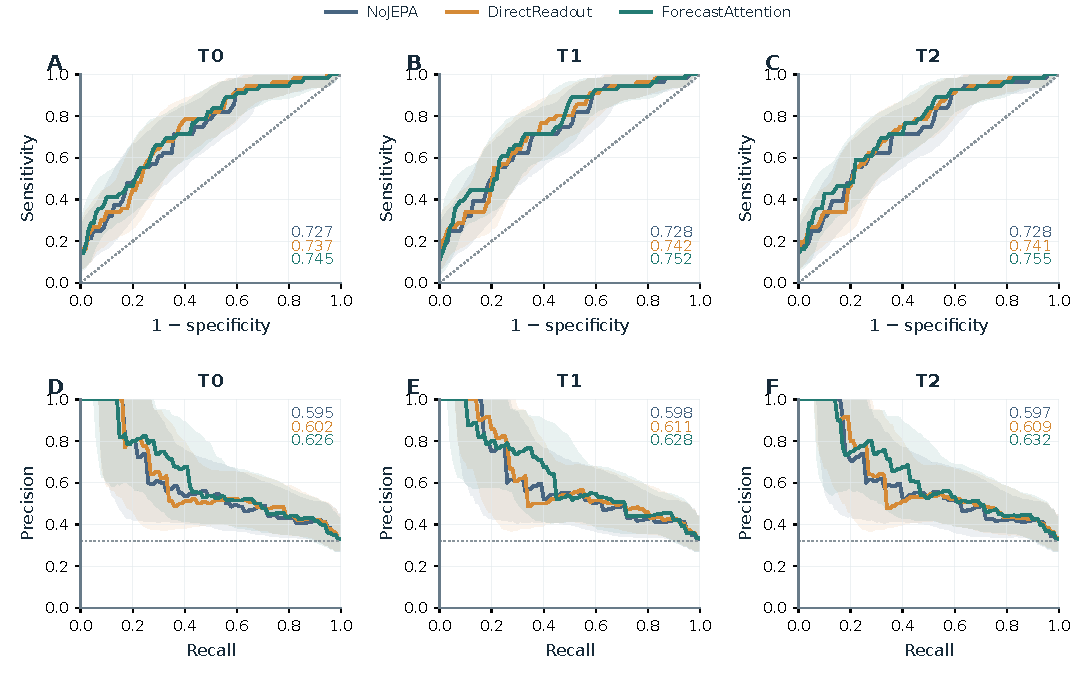
\includegraphics[width=\textwidth]{figures/discrimination.pdf}
\caption{Discrimination of seed-44 five-fold probability ensembles. (A--C) ROC curves; (D--F) precision--recall curves. Each patient's probabilities are averaged across the five fold models before constructing a curve or computing a metric. Shading shows pointwise 95\% paired patient-bootstrap intervals conditional on the fitted ensemble. Colored values give AUROC or non-interpolated AP calculated directly from ensemble scores; grid interpolation may change the plotted area. The dotted PR reference is the 0.32 positive prevalence.}
\label{fig:discrimination}
\end{figure*}

Under direct readout, adding future-state supervision increased macro AUROC by 0.0121, AP by 0.0107, and F1 by 0.0261. The complete forecast-attention readout gave a further AUROC increase of 0.0108 and AP increase of 0.0208, but a F1 decrease of 0.0074 relative to \direct{}. The first comparison more closely isolates auxiliary supervision; the second jointly changes forecast inputs, pooling, and classifier width. The supplementary \meanmodel{} achieved macro AUROC/AP/F1 of 0.7465/0.6139/0.5742 (Table~\ref{tab:pooling}). It therefore had higher F1 than the attention model, despite lower AUROC and AP. Attention did not produce a uniform improvement over mean pooling.

Paired patient intervals qualify these descriptive rankings (Fig.~\ref{fig:paired}). The macro AUROC difference for \fullmodel{} versus \nojepa{} was +0.0228 [0.0012, 0.0465]. The \direct{}--\nojepa{} difference was +0.0121 [$-0.0038$, 0.0287], and the \fullmodel{}--\direct{} difference was +0.0108 [$-0.0101$, 0.0327]. AP and F1 contrasts between the complete model and either direct control had intervals including zero. In particular, the full-versus-direct F1 difference was $-0.0074$ [$-0.0424$, 0.0352]. These intervals condition on a retrospectively selected seed and ensemble policy and exclude their selection uncertainty.

The paired DeLong test for the full-versus-\nojepa{} Macro AUROC difference gave a nominal two-sided $p=0.0462$, increasing to $p_{\mathrm{Holm}}=0.4161$ after adjustment over the nine principal Macro comparisons (Table~\ref{tab:bootstrap}). The corresponding raw/adjusted AUROC values were 0.1401/0.8404 for \direct{} versus \nojepa{} and 0.3055/1.0000 for \fullmodel{} versus \direct{}. None of the nine principal AUROC/AP/F1 comparisons met the adjusted 0.05 criterion. The unadjusted interval excluding zero for the complete-versus-control AUROC therefore does not establish a multiplicity-adjusted difference. These nonsignificant results do not demonstrate equivalence.
\begin{table*}[t]
\centering
\small
\caption{Exploratory principal Macro comparisons. AUROC uses paired DeLong tests with correlated landmark placements averaged per patient. AP and F1 use approximate, null-centered paired patient-bootstrap tests with 99,999 shared resamples. All $p$ values are two-sided. Holm adjustment covers all nine entries in this table. Direct and Attention abbreviate DirectReadout and ForecastAttention. $^{*}p_{\mathrm{Holm}}<0.05$, $^{**}p_{\mathrm{Holm}}<0.01$, $^{***}p_{\mathrm{Holm}}<0.001$; ns, not significant after the stated correction. Intervals are unadjusted 95\% patient-bootstrap intervals (2,000 shared draws) and need not agree with adjusted test decisions. All analyses condition on the fitted, retrospectively selected seed44 ensembles.}
\label{tab:bootstrap}
\begin{tabular}{llrrrc}
\toprule
Comparison & Metric & Difference [95\% CI] & $p$ & $p_{\mathrm{Holm}}$ & Sig. \\
\midrule
Direct -- NoJEPA & AUROC & +0.0121 [-0.0038, +0.0287] & 0.1401 & 0.8404 & ns \\
Direct -- NoJEPA & AP & +0.0107 [-0.0114, +0.0321] & 0.3286 & 1.0000 & ns \\
Direct -- NoJEPA & F1 & +0.0261 [-0.0039, +0.0621] & 0.1150 & 0.8048 & ns \\
Attention -- NoJEPA & AUROC & +0.0228 [+0.0012, +0.0465] & 0.0462 & 0.4161 & ns \\
Attention -- NoJEPA & AP & +0.0315 [-0.0030, +0.0698] & 0.0899 & 0.7190 & ns \\
Attention -- NoJEPA & F1 & +0.0188 [-0.0264, +0.0735] & 0.4471 & 1.0000 & ns \\
Attention -- Direct & AUROC & +0.0108 [-0.0101, +0.0327] & 0.3055 & 1.0000 & ns \\
Attention -- Direct & AP & +0.0208 [-0.0108, +0.0566] & 0.2327 & 1.0000 & ns \\
Attention -- Direct & F1 & -0.0074 [-0.0424, +0.0352] & 0.6995 & 1.0000 & ns \\
\bottomrule
\end{tabular}
\end{table*}


\begin{figure*}[t]
\centering
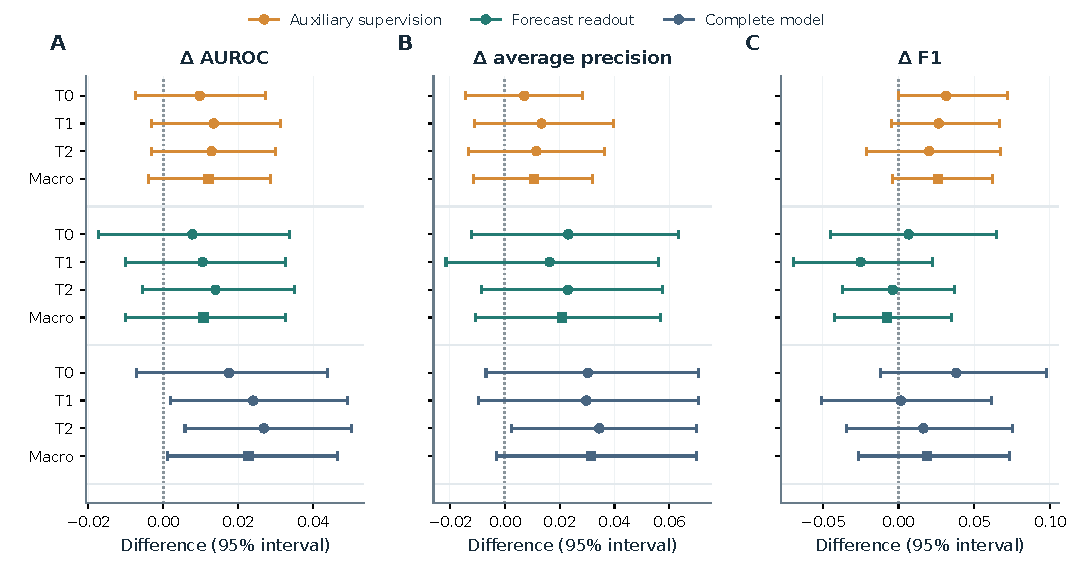
\includegraphics[width=\textwidth]{figures/paired_comparisons.pdf}
\caption{Paired differences between seed-44 ensembles at T0, T1, T2, and the landmark macro. Colors distinguish auxiliary supervision, additional forecast readout, and the complete-model contrast. Squares denote macro estimates. Bars are unadjusted 95\% patient-bootstrap intervals with identical patient draws shared across models and landmarks; adjusted tests are reported separately in Tables~\ref{tab:bootstrap} and~\ref{tab:significance_landmarks}. Five constituent fold models do not represent five independent test cohorts.}
\label{fig:paired}
\end{figure*}

\subsection{Threshold behavior and class imbalance}
\begin{table*}[t]
\centering
\small
\caption{Extended operating-point metrics for seed 44 at probability threshold 0.5. Each patient score is the arithmetic mean of probabilities from the five fold models before any metric is calculated. All landmarks contain the same 175 holdout patients (56 pCR-positive). Macro equally averages the three landmark metric values. PPV and NPV denote positive and negative predictive value; BA is balanced accuracy.}
\label{tab:extended_operating}
\begin{tabular}{llrrrrrr}
\toprule
Model & Stage & Sens. & Spec. & PPV & NPV & BA & MCC \\
\midrule
NoJEPA & T0 & 0.607 & 0.689 & 0.479 & 0.788 & 0.648 & 0.281 \\
NoJEPA & T1 & 0.625 & 0.681 & 0.479 & 0.794 & 0.653 & 0.289 \\
NoJEPA & T2 & 0.625 & 0.689 & 0.486 & 0.796 & 0.657 & 0.298 \\
NoJEPA & Macro & 0.619 & 0.686 & 0.481 & 0.793 & 0.653 & 0.289 \\
\midrule
DirectReadout & T0 & 0.643 & 0.706 & 0.507 & 0.808 & 0.674 & 0.331 \\
DirectReadout & T1 & 0.661 & 0.689 & 0.500 & 0.812 & 0.675 & 0.330 \\
DirectReadout & T2 & 0.679 & 0.664 & 0.487 & 0.814 & 0.671 & 0.321 \\
DirectReadout & Macro & 0.661 & 0.686 & 0.498 & 0.811 & 0.673 & 0.328 \\
\midrule
ForecastAttention & T0 & 0.661 & 0.697 & 0.507 & 0.814 & 0.679 & 0.339 \\
ForecastAttention & T1 & 0.714 & 0.571 & 0.440 & 0.810 & 0.643 & 0.267 \\
ForecastAttention & T2 & 0.714 & 0.613 & 0.465 & 0.820 & 0.664 & 0.306 \\
ForecastAttention & Macro & 0.696 & 0.627 & 0.471 & 0.814 & 0.662 & 0.304 \\
\bottomrule
\end{tabular}
\end{table*}

At threshold 0.5, \fullmodel{} had macro sensitivity 0.6964 and NPV 0.8145, compared with 0.6607 and 0.8113 for \direct{} (Table~\ref{tab:extended_operating}). These increases were accompanied by lower specificity (0.6275 versus 0.6863) and PPV (0.4705 versus 0.4981). The sensitivity difference was +0.0357 [$-0.0106$, 0.1006], while the specificity difference was $-0.0588$ [$-0.0948$, $-0.0234$]. The sensitivity interval therefore included zero even though the specificity decrease was more clearly separated from zero in this conditional analysis.

The full model's operating point varied across landmarks. At T0, it identified 37 positive outcomes and produced 36 false positives. At T1 it identified 40 positive outcomes but produced 51 false positives; at T2 it again identified 40 and produced 46 false positives. Thus the T0--T1 change yielded three additional true positives alongside 15 additional false positives, explaining why improved ranking could coexist with lower F1 at 0.5.

Among the principal models, \direct{} had the highest macro balanced accuracy (0.6735) and MCC (0.3277), compared with 0.6619 and 0.3038 for \fullmodel{} and 0.6527 and 0.2894 for \nojepa{}. Macro raw accuracy was 0.6781, 0.6495, and 0.6648, respectively. All were below the all-negative reference of 0.68 in this cohort. Accuracy alone would therefore obscure discrimination of the minority class. The supplementary \meanmodel{} reached accuracy 0.6838, balanced accuracy 0.6793, and MCC 0.3386.

OOF-selected Youden thresholds changed holdout F1 from 0.5416 to 0.5471 for \nojepa{}, 0.5678 to 0.5713 for \direct{}, and 0.5604 to 0.5631 for \fullmodel{} (Table~\ref{tab:extended_threshold}). For the full model, sensitivity increased to 0.7202 while specificity decreased to 0.6050. In contrast, \meanmodel{} F1 decreased from 0.5742 to 0.5563. These outcomes concern transfer of thresholds fitted on single-model OOF scores to ensemble scores. They neither optimize a holdout threshold nor establish calibration of the ensemble.

\subsection{Longitudinal information and probability quality}
The paired T2--T0 AUROC change was +0.0099 [0.0013, 0.0187] for \fullmodel{}, +0.0006 [$-0.0062$, 0.0070] for \nojepa{}, and +0.0038 [$-0.0064$, 0.0140] for \direct{}. For the full model, the corresponding AP change was +0.0059 [$-0.0098$, 0.0203] and F1 change was $-0.0103$ [$-0.0535$, 0.0340]. Its AUROC improvement therefore did not imply an improvement in every endpoint summary. Outcome-conditioned changes in each patient's ensemble score are shown in Fig.~\ref{fig:scorechanges}.

No comparison met the Holm-adjusted 0.05 criterion in the 81-test secondary family, which includes landmark, operating, probability-quality, pooling, and longitudinal comparisons (Tables~\ref{tab:significance_landmarks}--\ref{tab:significance_longitudinal}). For example, the full model's T2--T0 AUROC change had raw $p=0.0145$ but adjusted $p=1.0000$. The full-versus-direct specificity decrease had raw $p=0.00175$ and adjusted $p=0.14175$. Adjusting all 90 comparisons jointly also yielded no significant result. These tests qualify the descriptive trends without establishing absence of an effect.

\begin{table*}[t]
\centering
\small
\caption{Probability quality of the seed44 fivefold probability ensemble, averaged over T0--T2 metrics. Lower is better. ECE uses ten equal-width bins.}
\label{tab:calibration}
\begin{tabular}{lrrr}
\toprule
Model & NLL & Brier & ECE \\
\midrule
NoJEPA & 0.5822 & 0.2010 & 0.1337 \\
DirectReadout & 0.5819 & 0.2001 & 0.1272 \\
ForecastAttention & 0.5990 & 0.2061 & 0.1687 \\
\bottomrule
\end{tabular}
\end{table*}

Macro NLL/Brier/ECE was 0.5990/0.2061/0.1687 for \fullmodel{}, compared with 0.5819/0.2001/0.1272 for \direct{} and 0.5822/0.2010/0.1337 for \nojepa{}. The complete model's stronger ranking therefore coexisted with worse point estimates of all three probability-quality metrics. Its Brier score and ECE were worse at T1 and T2 than at T0, although AUROC increased across the three visits (Fig.~\ref{fig:longitudinal}). Reliability diagrams provide a complementary description of the ensemble probabilities (Fig.~\ref{fig:calutility}). All 14 macro metrics and their conditional patient intervals are reported in Table~\ref{tab:extended_macro}.

\begin{figure*}[t]
\centering
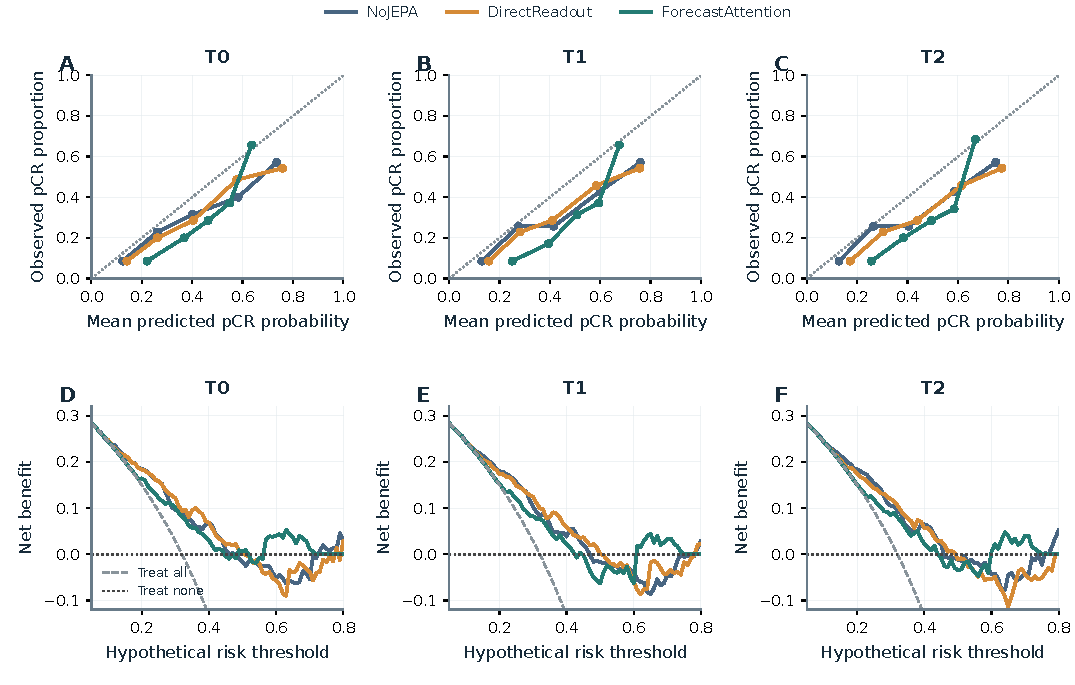
\includegraphics[width=\textwidth]{figures/calibration_utility.pdf}
\caption{Probability quality and hypothetical decision utility of the seed-44 ensembles. (A--C) Reliability diagrams use five equal-count ensemble-probability rank groups, each containing 35 patients; these differ from the ten fixed probability bins used for ECE. (D--F) Net-benefit curves for generic threshold-based positive actions with treat-all and treat-none references. Scores are five-fold mean probabilities without recalibration. No specific escalation or de-escalation strategy is validated.}
\label{fig:calutility}
\end{figure*}

\subsection{Hypothetical net benefit}
Decision curves did not preserve the discrimination ranking across thresholds. At a hypothetical risk threshold of 0.30, macro net benefit was 0.1222 for \direct{} and 0.0890 for \fullmodel{}. At threshold 0.50, all three principal models had negative macro net benefit: $-0.0152$, $-0.0019$, and $-0.0305$ for \nojepa{}, \direct{}, and \fullmodel{}, respectively. At 0.70 the ordering reversed, with +0.0279 for \fullmodel{} and $-0.0413$ for \direct{}. These threshold-dependent values use uncalibrated probabilities and a generic mathematical utility; they do not establish an acceptable clinical operating point.

\subsection{Exploratory biological and acquisition-related subgroups}
All four HR/HER2 groups had positive point estimates of the macro AUROC difference between \fullmodel{} and \nojepa{}, but every corresponding interval included zero (Fig.~\ref{fig:subgroups}; Table~\ref{tab:subgroups}). Differences were +0.0287 [$-0.0318$, 0.0914] in HR-positive/HER2-negative patients (68 patients, 11 positive), +0.0307 [$-0.0750$, 0.1318] in HR-positive/HER2-positive patients (31, 12 positive), +0.0748 [$-0.0251$, 0.2502] in HR-negative/HER2-positive patients (14, 7 positive), and +0.0331 [$-0.0128$, 0.0840] in HR-negative/HER2-negative patients (62, 26 positive). These small exploratory groups do not support a confirmed subtype-specific advantage or interaction.

Operating behavior also differed by group. In HR-positive/HER2-negative patients, the full model's macro sensitivity/specificity was 0.2424/0.9474, compared with 0.0909/0.9825 for \nojepa{}. Improved ranking therefore coexisted with low sensitivity at threshold 0.5. Age and source-namespace analyses are descriptive; the two namespaces belong to the same clinical release and do not constitute external validation. Only 11 patients had partial clipping of the largest predicted baseline component, including one positive outcome. AUROC and AP were suppressed for this group under the minimum-outcome rule.

\begin{figure*}[t]
\centering
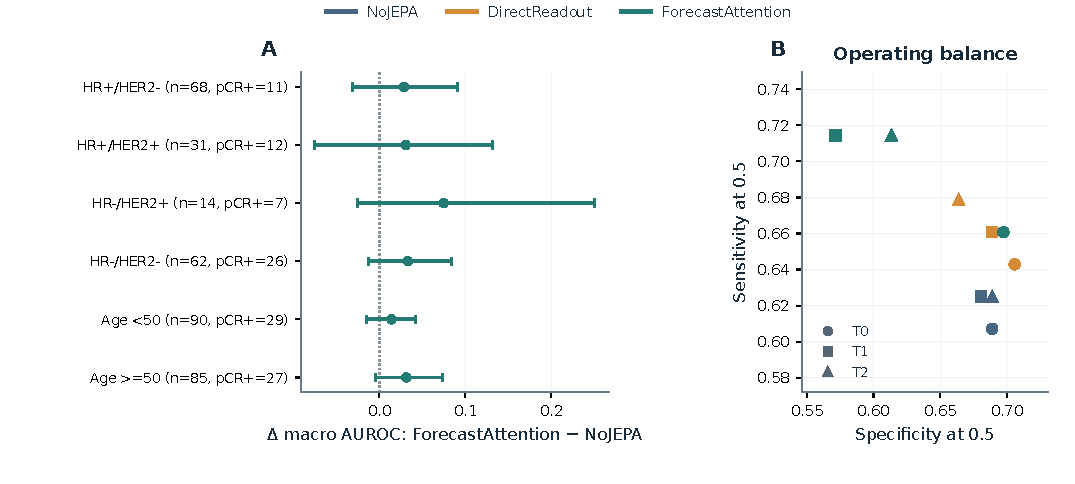
\includegraphics[width=\textwidth]{figures/subgroup_operating.pdf}
\caption{Exploratory subgroup and operating-point summaries from seed-44 ensemble probabilities. (A) Macro AUROC differences between ForecastAttention and NoJEPA within HR/HER2 and age groups, with sample sizes, positive outcomes, and unadjusted paired intervals. No subgroup-interaction claim is made. (B) Specificity and sensitivity at threshold 0.5 across landmarks; colors identify models and markers identify landmarks.}
\label{fig:subgroups}
\end{figure*}

\subsection{Archived forecast and gradient diagnostics}
Archived fixed-training-probe diagnostics provide a separate view of the five individual seed-44 models (Fig.~\ref{fig:mechanism}). At common epoch 20, fold-mean copy-normalized forecast skills for \direct{} were +0.0258, +0.0500, and +0.1935 at one-, two-, and three-step horizons. Corresponding values for \fullmodel{} were $-0.0368$, $-0.0154$, and +0.0242 (Table~\ref{tab:worldprobe}). Each skill is normalized within its own snapshot's EMA coordinates and then averaged across folds; latent states from separate models are not ensembled. The complete model's better pCR ranking cannot simply be attributed to uniformly more accurate latent forecasts under this diagnostic.

The diagnostic requires the real landmark, target, and every intermediate visit, whereas the training objective masks unavailable future targets. Its eligible populations therefore vary by horizon. Only 5--9 patients per training probe were eligible at three steps, and these are not best-checkpoint holdout forecast measurements. The predictor's pCR-loss gradient norm was zero for \direct{} and averaged 0.7148 for \fullmodel{}; weighted rollout-gradient norms were 0.1213 and 0.1308. These values support the expected gradient routing, but gradient magnitude is not a biological effect size. \nojepa{} has no available trained-world diagnostic and is not assigned an artificial zero skill.

\begin{figure*}[t]
\centering
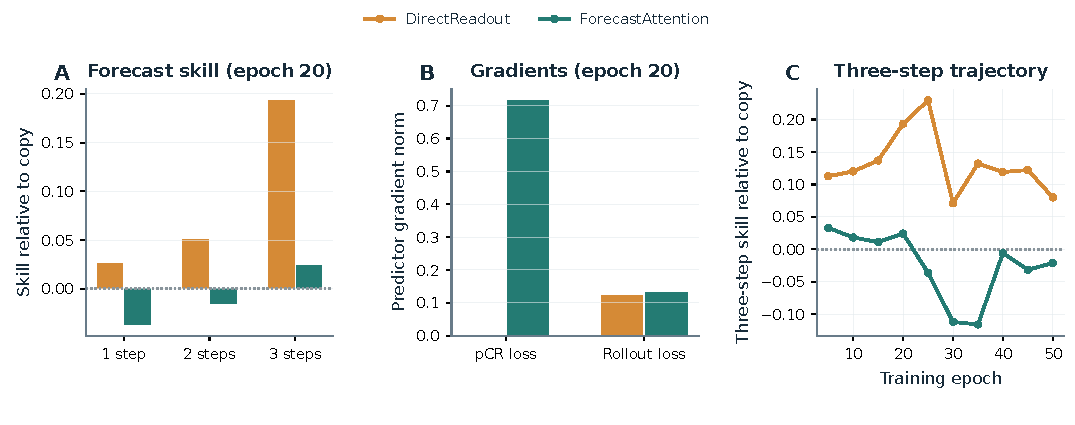
\includegraphics[width=\textwidth]{figures/forecast_mechanism.pdf}
\caption{Archived seed-44 fixed-training-probe diagnostics. (A) Copy-normalized forecast skill at common epoch 20. (B) Predictor gradient norms from pCR and weighted rollout losses. (C) Three-step skill across common archived epochs. Statistics are computed within each model's EMA coordinates and averaged across five folds, distinct from probability ensembling for pCR. These are training diagnostics; real continuous visit chains are required and three-step eligibility is only 5--9 patients per probe.}
\label{fig:mechanism}
\end{figure*}
